\documentclass[12pt,conference,twocolumn]{IEEEtran}
\usepackage{diagbox}
\usepackage{graphicx}
\usepackage{amsmath}
\usepackage{amsfonts}
\usepackage{algpseudocode}
\usepackage{algorithm}
\usepackage{subfigure}
\usepackage{tikz}
% \usepackage[linesnumbered,ruled,vlined]{algorithm2e}
\usepackage{epsfig}
% \usepackage{pst-grad} % For gradients
% \usepackage{pst-plot} % For axes
\usepackage{cite}
\usetikzlibrary{shapes}
\usetikzlibrary{arrows,automata}
\usetikzlibrary{positioning}
\usetikzlibrary{patterns}
\usetikzlibrary{backgrounds}
\newtheorem{theorem}{Theorem}
\newtheorem{proof}{Proof}
\newtheorem{proposition}{Proposition}
\newtheorem{definition}{Definition}
\newtheorem{lemma}{Lemma}
\newtheorem{corollary}{Corollary}
\newtheorem{example}{Example}

%\renewcommand{\baselinestretch}{1}

\renewcommand{\ae}[1]{{\color{red}{#1}}}
\newcommand{\my}[1]{{\color{blue}{#1}}}
\newcommand{\old}[1]{{\color{green}{#1}}}
\begin{document}  
\title{Schedulability Analysis for Dual Priority Scheduling}  
\maketitle  


% According to Baruah (2003, Dynamic- and Static-priority Scheduling of Recurring Real-time Tasks, Theorem~3), $\tau_i$ is schedulable on a single processor using static priority if and only if for each absolute deadline of a job  $d_{i,k}$ where $k\in N$, there exists an interval $d_{i,k-1}\leq t'\leq d_{i,k}$ for which the following condition holds:
% \begin{equation}
% dbf(\tau_i,t)+\sum_{\tau_j\in\{hp_i\}}rbf_i(\tau_j,t')\leq t'	
% \end{equation} 

% Here the demand bound function captures the maximum execution demand of $\tau_i$ for a time interval length $t$ if it is to meet all deadlines.
% \begin{equation}
% dbf(\tau_i,t)=\left(\lfloor \frac{t-D_i}{T_i}\rfloor+1\right)\times C_i
% \end{equation} 


% On the other hand, the request bound function  $rbf_i(\tau_j,t')$ denotes the maximum amount of time for which $\tau_j$ could \textbf{deny the processor} to lower priority task $\tau_i$ over some interval length of $t'$. \\\\



\section{Dual Priority}
Given a task system $\tau=\{\tau_1,\tau_2,\ldots, \tau_n\}$, we first make the following \textbf{assumptions}:
\begin{enumerate}
	\item Each task  $\tau_i$ has a original priority $n+i$ and a promotion priority $i$.
	\item Each task has a fixed promotion point $p_i$. The concerned job $J_{i,k}$ has its promotion point $P_i=r_{i,k}+p_i$.
\end{enumerate}

\my{
\begin{lemma}[Worst Case  Pattern]
\label{lemma:pattern}
Suppose $\tau$ could experience deadline miss with the current priority and promotion point  assignment, then it must be that there exists a busy time interval $[0,t]$  during  which some job of task $\tau_i\in\tau$ would miss its deadline when all other tasks  release their first job at time instant $0$, and all jobs including those released by $\tau_i$ are released as soon as possible with corresponding period.
\end{lemma}
\begin{proof}
Among all possible legal event sequences in which $\tau$ misses some deadline,  let $S$ denote such a sequence where some job of $\tau_i\in \tau$  misses its deadline within the shortest busy interval $[0,t_F]$.  As a result no deadline miss would happens earlier than $t_F$. 

Assuming in the event sequence $S$, there exists some tasks, e.g.,  $\tau_j$ whose first release is not at time instant $0$ and the separation between some job release is greater than  $T_j$. Then as we shift $r_{j,1}$ to $0$ and reduce  time separation  between each job releases to $T_j$, $\tau_i$ would consume no more resource than before.

This is because that all jobs of $\tau_j$ with deadline before $t$ would still meet its deadline (otherwise we can construct a new sequence $S$), while the last job of $\tau_j$ released before $t$ (e.g., $J_{j,m}$) is more likely to  deny processor from $\tau_i$ since the promotion point of job $J_{j,m}$ will also decrease. Therefore after we modify the release pattern of $\tau_j$, $\tau_i$ would still misses its deadline. Finally by repeating the above steps for all such tasks, the deadline miss of $\tau_i$ would still happen at $t_F$. Therefore Lemma 1 is true.
\end{proof}
\begin{figure}[h!]
 \centering
\includegraphics[scale=0.7]{Figure/WC}  
\caption{Worst Case  Pattern}
  \label{fig:case2}
\end{figure}
From Lemma~\ref{lemma:pattern} we know that if $\tau$ would  experience some deadline miss, then there exists a $\tau_i$ that will have its  deadline miss with the worst case release pattern defined in Lemma~\ref{lemma:pattern}. Therefore the following corollary can tell us whether a task system $\tau$ is schedulable by the dual priority scheduling algorithm.

\begin{corollary}
\label{corollary:condition}
If  $\forall \tau_i\in \tau$ no deadline miss happens for all possible time interval length $t$ with the worst case release pattern:  1) some job of $\tau_i$ has deadline at $t$  and all jobs of $\tau_i$ are released as soon as possible  with period $T_i$; 2) first job of $\tau_j\in \tau-\tau_i$ is released at $0$ and all jobs are released as soon as possible with period $T_j$, then $\tau$ is schedulable by the dual priority scheduling algorithm.
\end{corollary}
\begin{proof}
This corollary is a direct deduction from Lemma~\ref{lemma:pattern}.
\end{proof}


From Corollary~\ref{corollary:condition}, we know  that as along as we can guarantee that $\forall~\tau_i\in \tau:~\forall~t:$ no deadline miss happens with the worst case release pattern,  then we can declare that the task system $\tau$ is schedulable by the dual priority scheduling algorithm. Therefore  in the simplest case,  an exact but computational expensive schedulability test for dual priority scheduling algorithm could be derived by simulating the behavior of the system with the worst case release pattern. 


To reduce the complexity, we need a more efficient test to determine whether $\tau_i\in\tau$ is schedulable when jobs are released with the worst case release in Lemma~\ref{lemma:pattern}. Let $ibf_i(\tau_j,t')$ (ibf is short for interference bound function) denote maximum possible resource consumed by $\tau_j\in\tau-\tau_j$ in the system  during the time interval $[0,t']$, and let $dbf(\tau_i,t)$ denotes the maximum execution requirement of $\tau_i$ during $[0,t]$,  when all tasks are released with worst case pattern in Lemma~\ref{lemma:pattern}.\footnote{Note that the two functions are specific for the worst case pattern.}  Therefore the following theorem can be used to determine whether $\tau_i\in \tau$ is schedulable when all jobs in the system is released in the worst case release pattern.
}
\begin{theorem}
\label{theorem:1}
$\tau_i$ would not experience any deadline miss with the worst case release pattern on a single processor by the dual priority scheduling algorithm if the following condition holds:
\begin{equation}
\label{eq:1}
\forall~t~:\exists~t'\in[t-D_i, t]:~dbf(\tau_i,t)+ibf_i(\tau-\tau_i,t')\leq t'
\end{equation} 
where \[ibf_i(\tau-\tau_i,t')=\sum_{\tau_j\in \tau-\tau_i}ibf_i(\tau_j,t')\].
\end{theorem}
\begin{proof}
We can prove the statement that if $\tau_i$ is not schedulable with the worst case release pattern, then Equation~\ref{eq:1} would not hold. Suppose that $\tau_i$ is not schedulable then there are legal event sequences in which $\tau_i$ misses some deadline when $\tau_i$ is assigned with the current priority and promotion point. Let $S'$ denote such a sequence where $\tau_i$ misses deadline at the earliest time at $t$.

It must be the cases that during $[0,t]$ some tasks are executing because otherwise the time interval between the last idle instant to $t$ could also construct such a sequence. Then it must be that during the time interval $[0,t']$, other tasks have consumed an amount of resource more than 
\[
ibf_i(\tau-\tau_i,t')>t'-dbf(\tau_i,t)
\]
which contradicts the Equation~\ref{eq:1}.
\end{proof}
With Theorem~\ref{theorem:1}, we can use the following test to whether a task system $\tau$ is schedulable by the dual priority scheduling algorithm.
\begin{theorem}
A task system $\tau$ is schedulable by the dual priority scheduling on unit-speed uniprocessor if the following hold: $\forall \tau_i\in \tau:~\forall~t:~\exists~t'\in[t-D_i, t]:~$
\begin{equation}
dbf(\tau_i,t)+ibf_i(\tau-\tau_i,t')\leq t'
\end{equation}
\end{theorem}



In the worst case release pattern, we can easily calculate the exact value of $dbf(\tau_i,t)$. However the exact value of $ibf_i(\tau-\tau_i,t')$ is not trivial except we simulate the system.  As a result, here we use an upper bound of the actual interference to represent  $ibf_i(\tau_j,t')$ instead.





% \begin{example}
% As shown in the Figure~1, when $r_i\leq t'\leq P_i$, the execution requirement of $J_{j,k}$ is $C_j$ because $\tau_i$  would execute only after $J_{j,k}$ finishes. However, when $P_i\leq t'\leq P_j$,  the time $J_{j,k}$ deny processor from $\tau_i$ is equal the time that $J_{j,k}$ has already executed, because $\tau_i$ has higher priority than $\tau_j$ during $[P_i,P_j]$.  This is a significantly different from the  static priority scheduling.
% \begin{figure}[h!]
%  \centering
% 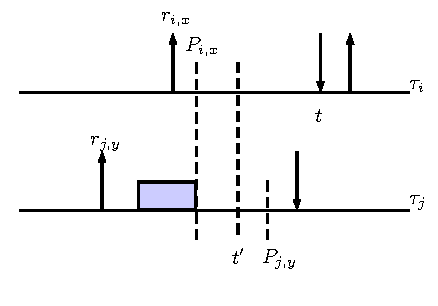
\includegraphics[scale=1]{Figure/E1}  
% \caption{Example One}
%   \label{fig:p3}
% \end{figure}
% \end{example}

% Unfortunately, it is hard to calculate the exact time that  $J_{j,k}$  has executed, and therefore here instead,  we would use an upper bound of the resource $J_{i,k}$ has consumed to derive the test.





Here we first present some notations that  will be used later in the paper.
\begin{table}[h]
\caption{Notations}
\label{tab:x}
\center
\begin{tabular}{|l|l|l|l|}
 \hline
 $m=\lfloor \frac{t'}{T_j}\rfloor$ & $r_{j,m}=m\times T_j$ &$P_{j,m}=m\times T_j+p_j$ \\
 \hline
$P_{i,n}=t-D_i+p_i$ & $r_{i,n}=P_{i,n}-p_i$ &$[a]_0=\max(a,0)$\\
 \hline
$m'=\lfloor \frac{r_i}{T_j}\rfloor$  & $r_{j,m'}=m'\times T_j$& \\
 \hline
	$m''=\lfloor \frac{P_{i,n}}{T_j}\rfloor$ &  $r_{j,m''}=m''\times T_j$&	\\
  \hline
\end{tabular}
\end{table}

\section{Schedulability Test}


% Here we also derive $rbf_{i}^1(\tau_j,t')$ which denotes \ae{maximum possible} execution that $\tau_j$ has received after $r_i$,  and $rbf_{i}^2(\tau_j,t')$ which denotes \ae{maximum possible} execution  that $\tau_j$ has received after $P_i$ (if $t'>P_i$).  Assuming no deadline miss happens earlier, the total execution before $r_i$ and $P_i$ should not exceed $r_i$ and $P_i$, respectively. As a result, we are able to tighten the schedulability test by bounding the total execution before $r_i$ and $P_i$ by $r_i$ and $P_i$, respectively.




% \subsection{$rbf_i(\tau_j,t')$ when $j<i$}
% \begin{figure}[h!]
%  \centering
% 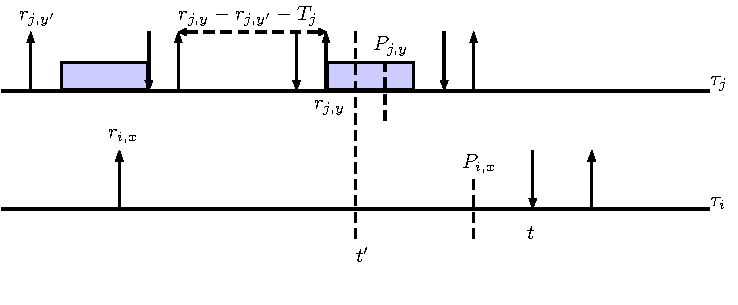
\includegraphics[scale=1]{Figure/C1}  
% \caption{$ P_j\leq P_i$}
%   \label{fig:case1}
% \end{figure}
% \textbf{Case 1 ( $P_j\leq P_i$)~as shown in  Figure~\ref{fig:case1}:} 

% The promotion point of $P_i$ is greater than $P_j$, and hence $\tau_i$ always has lower priority than $\tau_i$. Thus its maximum possible execution units by $t'$ is 

% 	\begin{align*}
% 		rbf_i(\tau_j,t')=n_j.C_j +\min(C_j,t'-r_j)
% 	\end{align*}
% Its maximum possible execution after $r_i$ is
% 	\begin{align*}
% 	\begin{split}
% 	rbf_{i}^1(\tau_j,t')=
% 	\begin{cases}
% 	\min\{C_j, t'-r_i\}&\mbox{if } r_j\leq r_i\\
% 	\min\{C_j, t'-r_j\}+\frac{r_j-r_j^s-T_j}{T_j}C_j+\min(C_j,[r_j^s+D_j-r_i]_0)  &\mbox{if } r_j>r_i
% 	\end{cases}
% 	\end{split}
% 	\end{align*}
% Its maximum possible execution after $P_i$ is
% 	\begin{align*}
% 	\begin{split}
% 	rbf_{i}^2(\tau_j,t')=
% 	\begin{cases}
% 	\min\{C_j, [t'-P_i]_0\}&\mbox{if } r_j\leq P_i\\
% 	\min\{C_j, t'-r_j\}+\frac{r_j-r_j^w-T_j}{T_j}C_j+\min(C_j,[r_j^w+D_j-P_i]_0)  &\mbox{if } r_j>P_i
% 	\end{cases}
% 	\end{split}
% 	\end{align*}





% \begin{figure}[h!]
%  \centering
% \includegraphics[scale=1]{Figure/C2}  
% \caption{$P_j> P_i$}
%   \label{fig:case2}
% \end{figure}

% \textbf{Case 2 ( $P_j> P_i$)~as shown in  Figure~\ref{fig:case2}} $\tau_i$ has higher priority than $\tau_j$'s last job during $[\max(r_j,P_i),P_j]$ if $P_i\leq P_j$:
% 	\begin{align*}
% 		rbf_i(\tau_j,t')=\lfloor \frac{t'}{T_j} \rfloor C_j +\min\left(C_j,t'-r_j-\left(\min\{t',P_j\}-\max\{r_j,P_i\}\right)\right)
% 	\end{align*}
% Its maximum possible execution after $r_i$ is
% \begin{align*}
% \begin{split}
% rbf_{i}^1(\tau_j,t')=
% \begin{cases}
% \min\{C_j,\min\{t',P_i\}-r_i\}&\mbox{if } t'<P_j\wedge r_j\leq r_i\\
% \min\{C_j,\min\{t',\max(r_j,P_i)\}-r_j\} +\frac{r_j-r_j^s-T_j}{T_j}C_j &	\\+\min(C_j,[r_j^s+D_j-r_i]_0)&\mbox{if } t'<P_j\wedge r_j> r_i\\
% \min\{C_j,t'-r_i-(P_j-P_i)\}&\mbox{if } t'\geq P_j\wedge r_j\leq r_i\\
% \min\{C_j,t'-r_j-(P_j-\max(r_j,P_i))\}+\frac{r_j-r_j^s-T_j}{T_j}C_j&\\ +\min(C_j,[r_j^s+D_j-r_i]_0)&\mbox{if } t'\geq P_j\wedge r_j> r_i\\
% \end{cases}
% \end{split}
% \end{align*}
% Its maximum possible execution after $P_i$ is
% \begin{align*}
% \begin{split}
% rbf_{i}^2(\tau_j,t')=
% \begin{cases}
% 0&\mbox{if } t'<P_j \wedge r_j\leq P_i\\
% \frac{r_j-r_j^w-T_j}{T_j}C_j+\min(C_j,[r_j^w+D_j-P_i]_0)&\mbox{if } t'<P_j \wedge r_j> P_i\\
% \min\{t'-P_j,C_j\}&\mbox{if } t'\geq P_j \wedge  r_j\leq P_i\\
% \min\{t'-P_j,C_j\}+\frac{r_j-r_j^w-T_j}{T_j}C_j+\min(C_j,[r_j^w+D_j-P_i]_0)&\mbox{if } t'\geq P_j \wedge  r_j> P_i\\
% \end{cases}
% \end{split}
% \end{align*}


% % %




% \subsection{$rbf_i(\tau_j,t')$ when $j> i$}
 


% \textbf{Case 1.1 ($P_i\leq P_j\wedge r_j\leq r_i$)~as shown in  Figure~\ref{fig:case3}}: $\tau_j$ may execute during $[r_j,r_i]$, and $\tau_j$ would not execute after $r_j$ or $P_i$ unless $\tau_i$ has finished.


% % However we should assume all deadlines before $t'$ is meet. whether we should assume it is meet.
% 	\begin{figure}[h!]
%  \centering
% 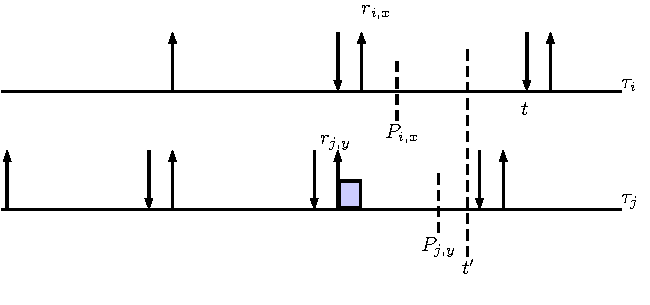
\includegraphics[scale=1]{Figure/C3}  
% \caption{$P_i\leq P_j\wedge r_j\leq r_i$}
%   \label{fig:case3}
% \end{figure}
% 		\begin{align*}
% 		rbf_i(\tau_j,t')=(\lfloor \frac{t'}{T_j} \rfloor)\times C_j+\min(C_j,r_i-r_j)
% 	\end{align*}
% \begin{align*}
% \begin{split}
% rbf_{i}^1(\tau_j,t')=rbf_{i}^2(\tau_j,t')=0
% \end{split}
% \end{align*}


% \textbf{Case 1.2 ($P_i\leq P_j\wedge r_j> r_i$)~as shown in  Figure~\ref{fig:case4}}:  the last job of $\tau_j$ would not execute unless $\tau_i$ finishes. However all previous jobs are assumed to finish because otherwise the deadline miss should be already found. The $n_j-1$ job must already finish by $\min(P_i,r_j-T_j+D_j)$.

% 	\begin{figure}[h!]
%  \centering
% 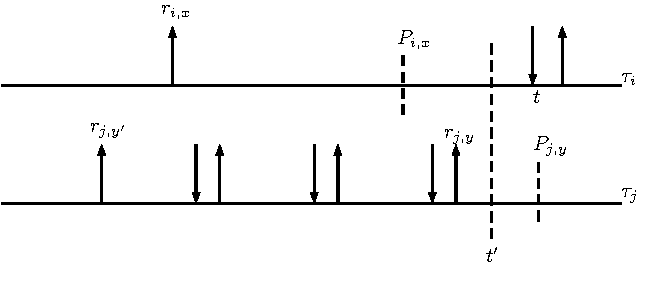
\includegraphics[scale=1]{Figure/C31}  
% \caption{$P_i\leq P_j\wedge r_j> r_i$}
%   \label{fig:case4}
% \end{figure}

% 	\begin{align*}
% 		rbf_i(\tau_j,t')=(n_j)\times C_j
% 	\end{align*}
% \begin{align*}
% \begin{split}
% rbf_{i}^1(\tau_j,t')&=\min(C_j, [\min(P_i,r_j-T_j+D_j)-r_i]_0)\\
% rbf_{i}^2(\tau_j,t')&=0
% \end{split}
% \end{align*}

% % \my{


% \textbf{Case 2.1 ($P_i>P_j\wedge r_j\leq r_i$)~as shown in  Figure~\ref{fig:case5}}:the last job of $\tau_j$ can execute until $\min(t',P_i)$
% 	\begin{align*}
% 		rbf_i(\tau_j,t')=(n_j) C_j+\min\left(C_j,r_i-r_j+[\min(t',P_i)-\max(P_j,r_i)]_0\right)
% 	\end{align*}
% 	\begin{align*}
% \begin{split}
% rbf_{i}^1(\tau_j,t')=\min\{C_j,[\min(t',P_i)-\max(P_j,r_i)]_0\}
% \end{split}
% \end{align*}
% \begin{align*}
% \begin{split}
% rbf_{i}^2(\tau_j,t')=0
% \end{split}
% \end{align*}

% \begin{figure}[h!]
%  \centering
% 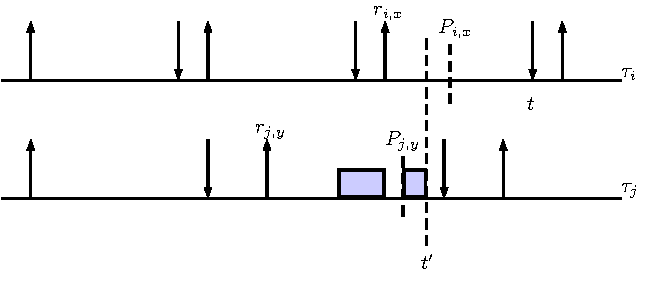
\includegraphics[scale=1]{Figure/C4}  
% \caption{$P_i>P_j\wedge r_j\leq r_i$}
%   \label{fig:case5}
% \end{figure}

% \begin{figure}[h!]
%  \centering
% 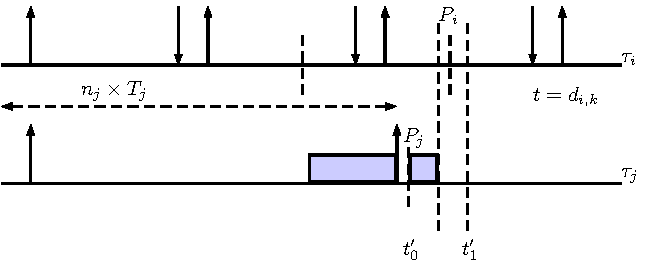
\includegraphics[scale=1]{Figure/C41}  
% \caption{$P_i>P_j\wedge r_j> r_i $}
%   \label{fig:case6}
% \end{figure}

% \textbf{Case 2.2 ($P_i>P_j\wedge r_j> r_i$)~as shown in  Figure~\ref{fig:case6}}: 
% \begin{align*}
% 	rbf_i(\tau_j,t')=(n_j) C_j+\min\left(C_j,[\min(t',P_i)-P_j]_0\right)
% \end{align*}


% \begin{align*}
% rbf_{i}^1(\tau_j,t')=\min\left(C_j,[\min(t',P_i)-P_j]_0\right)+\min(C_j,[r_j-T_j+D_j-r_i]_0)
% \end{align*}

% \begin{align*}
% rbf_{i}^2(\tau_j,t')=0
% \end{align*}





% \section{Optimization Technique}
% We can bound the total execution before $r_i$ or $P_i$ (if $t'>P_i$) by $r_i$ or $P_i$, respectively. For $\tau_i$ itself, we simply assume its execution demand after $r_i$ and $P_i$ is $C_j$.

% \begin{equation}
% F_1(\tau_i,t,t')=\min\left(r_i,n_i\times C_i+\sum_{\tau_j\in\{\tau-\tau_i\}}rbf_i(\tau_j,t')-rbf_{i}^1(\tau_j,t')\right)+\sum_{\tau_j\in\{\tau-\tau_i\}}rbf_{i}^1(\tau_j,t')+C_i
% \end{equation}


% \begin{equation}
% F_2(\tau_i,t,t')=\min\left(P_i,n_i\times C_i+\sum_{\tau_j\in\{\tau-\tau_i\}}rbf_i(\tau_j,t')-rbf_{i}^2(\tau_j,t')\right)+\sum_{\tau_j\in\{\tau-\tau_i\}}rbf_{i}^2(\tau_j,t')+C_i
% \end{equation}

% \begin{equation}
% \begin{split}
% F(\tau_i,t,t')=
% \begin{cases}
% F_1(\tau_i,t,t')&\mbox{if } t'<=P_i\\
% \min\{F_1(\tau_i,t,t'),F_2(\tau_i,t,t')\}&\mbox{otherwise}
% 	\end{cases}	
% \end{split}
% \end{equation}




% We can derive a simple upper bound of $t$. Suppose that
% \[
% \forall~t'\in(k.T_i,k.T_i+D_i]:~F(\tau_i,t,t')>t'\Rightarrow\min_{t'\in(k.T_i,k.T_i+D_i]}\frac{F(\tau_i,t,t')}{t'}>1
% \]
% , and let
% \[
% H_i(t)=  U\times t+\sum_{\tau_j\in\{\tau-\tau_i\}}C_j\geq t\times u_i+(\lfloor \frac{t'}{T_j} \rfloor+1)C_j\geq F(\tau_i,t,t')
% \]

% then it must be that

% \begin{align*}
% \frac{H_i(t)}{t-D_i}>1\Rightarrow t-D_i< U\times t+\sum_{\tau_j\in\{\tau-\tau_i\}}C_j\Rightarrow t<\frac{D_i+\sum_{\tau_j\in\{\tau-\tau_i\}}C_j}{1-U}
	
% \end{align*}

% \section{Draft Simulation Results}

% \begin{table}[h]
% \caption{Notations}
% \label{tab:x}
% \large
% \center
% \begin{tabular}{|l|l|l|l|l|}
%  \hline
% Uniform Distribution&[0.88,0.9]&[0.93,0.95]&[0.95,0.97]&[0.97,0.99]\\
%  \hline
% Acceptance Ratio&1&1&0.995&0.982\\
%  \hline
% \end{tabular}
% \end{table}
\end{document}  